\documentclass[a4paper]{article}

% Encoding
\usepackage[utf8]{inputenc} % Required for inputting international characters
\usepackage[T1]{fontenc} % Output font encoding for international characters

% Bilbliography
\usepackage[style=numeric,natbib=true,giveninits=true,sorting=none]{biblatex}

% Document class "MasterDoctoralThesis" internals
\usepackage[autostyle=true]{csquotes} % Required to generate language-dependent quotes in the bibliography
\usepackage{import}
\usepackage{tocbibind}

% Images
\usepackage{graphicx} % Permet l'insertion d'image (entre autres)
\usepackage{pict2e} % Pour faire des graphiques

% Tikz and colors
\usepackage{color}
\usepackage{xcolor}
\usepackage{tikz}
	\usetikzlibrary{patterns}
	\usetikzlibrary{plotmarks}
	\usetikzlibrary{calc}
	\usetikzlibrary{shapes}
	\usetikzlibrary{arrows}
	\usetikzlibrary{fadings}

% Maths
\usepackage{amsmath} % Mathematical environnements
\usepackage{amsfonts} % Mathematical fonts
\usepackage{amssymb} % Mathematical symbols

% Tables and figures
\usepackage{array} % For tables
\usepackage{floatrow} % ??
\usepackage{subfig} % Subfigure possible
\usepackage{tabu} % Better tabular

% Misc
\usepackage[english]{babel}
\usepackage{verbatim} % Verbatim
\usepackage{bbm} % Extended blackboard bold symbols
\usepackage[colorinlistoftodos, obeyFinal]{todonotes}
\usepackage{xspace} % Trailing space for custom commands
\usepackage{hyperref}
\hypersetup{
    colorlinks,
    linkcolor={red!50!black},
    citecolor={blue!50!black},
    urlcolor={blue!80!black}
}

% Showlabel
\usepackage{showlabels}

\renewcommand{\showlabelfont}{\tiny\color{blue}}
\renewcommand{\showlabelsetlabel}[1]{\colorbox{lightgray}{\showlabelfont #1}}

% Setup
\floatsetup[figure]{style=plain,subcapbesideposition=top}
\newcommand{\bigO}[1]{\mathcal{O}\left(#1\right)} % big O notation
\newcommand{\code}[1]{\texttt{#1}} % shortcut to insert code inline
\newcommand{\EE}[1]{\cdot 10^{#1}} % power of 10
\newcommand{\missingref}{[\todo[color=blue!30, size=\tiny, caption={Missing reference}]{Missing ref}?]\xspace}
\newcommand{\myvec}[1]{\boldsymbol{\mathrm{#1}}} % bold vectors
\newcommand{\norm}[1]{\Vert #1\Vert} % norm of a vector
\newcommand{\set}[1]{\{#1\}} % set notation with curly braces
\newcommand{\total}{\text{d}} % d for total derivative


% Project specific

\newcommand{\lambdavec}{\myvec{\lambda}}
\newcommand{\uvec}{\myvec{u}}

\makeatletter

\def\@setref#1#2#3{%
  \ifx#1\relax
   \protect\G@refundefinedtrue
   \nfss@text{\reset@font\bfseries\tiny\textcolor{red}{Ref to \colorbox{lightgray}{\texttt{#3}}}}%
   \@latex@warning{Reference `#3' on page \thepage \space
             undefined}%
  \else
   \expandafter#2#1\null
  \fi}

\makeatother

\title{Boundary condition}
\author{Benoît Richard \and Guiyuan Shi}

\begin{document}

\listoftodos

\maketitle

\abstract{\todo[inline]{Write abstract}}

\section{Introduction}

\todo[inline]{Write introduction}

\section{Giant viable cluster}

Consider a multiplex network with $L$ layers. Let $g_0^{(i)}$ and $g_1^{(i)}$ be the generating functions of respectively the degree and the excess degree in layer $i$. Moreover define $u_i$ as the probability that a vertex reached after following an edge in layer $i$ is not part of the giant viable cluster. Then if we pick a vertex $v$ at random the probability $S$ that it is part of the giant viable cluster can be written as
\begin{align}
	S &= P_0\left(\bigcap_{i = 1}^{L} \exists w \in N_i(v) \; w \in GVC \right).
\end{align}
By requiring that the layers are independent from one others, we can rewrite $S$ as a product
\begin{align}
	S &= \prod_{i = 1}^{L}  P_0\left(\exists w \in N_i(v) \; w \in GVC\right) \\
		&=\prod_{i = 1}^{L}  \left[1 - P\left(w \notin GVC \; \forall w \in N_i(v)\right) \right] \\
		&=\prod_{i = 1}^{L}  \left[1 - \sum_{k = 0}^{\infty} P\left((w \notin GVC \; \forall w \in N_i(v) | deg(v) = k \right) p^{(i)}_k \right] \\
		&=\prod_{i = 1}^{L}  \left[1 - \sum_{k = 0}^{\infty} u_i^k p^{(i)}_k \right] \\
		&=\prod_{i = 1}^{L}  \left[1 - g_0^{(i)}(u_i) \right].\label{Multiplex GCC size final}
\end{align}

We can find $u_j$ by a similar reasoning. First note that $1 - u_j$ is the probability that a vertex reached by following an edge in layer $j$ is in the giant viable cluster. Which as before can be written in the form
\begin{align}
	1 - u_j &= P_1^{(j)}\left(\bigcap_{i = 1}^{L} \exists w \in N_i(v) \; w \in GVC\right)\\
	&= \prod_{i = 1}^{L}  P_1^{(j)}\left(\exists w \in N_i(v) \; w \in GVC \right).
\end{align}
Since the layers are independent, the fact that we reached $v$ by following an edge in layer $j$ to reach vertex $v$ is irrelevant in all other layers. However in layer $j$ this means that the degree distribution follows the distribution $q_k^{(j)}$ rather than $p_k^{(j)}$. Putting this together we get
\begin{align}
	1 - u_j &= \left[1 - \sum_{k = 0}^{\infty} u_j^k q_k^{(j)} \right] \prod_{\substack{i = 1 \\ i \neq j}}^{L}  \left[1 - \sum_{k = 0}^{\infty} u_i^k p^{(i)}_k \right] \\
	&= \left[1 - g_1^{(j)}(u_j) \right] \prod_{\substack{i = 1 \\ i \neq j}}^{L}  \left[1 - g_0^{(i)}(u_i) \right]. \label{Multiplex u final}
\end{align}

\todo[inline]{Is this section too precise and should the results be given with just a citation ?}

\section{Boundary condition}

\subsection{General case}

Up to now, we have considered the multiplex generated to be determined via the degree distributions of each of its layer. However a degree distribution has an infinite number of degrees of freedom, therefore it is more practical to let the degree distributions depend on a finite set of parameters $\lambda_1, \lambda_2, \dots, \lambda_N$ and express the behaviour of the network in term of them. Note that the number of parameters $N$ does not need to match the number of layers $L$.

In order to make our main statement about the critical region for a multiplex network, we first need to introduce several quantities. First, let introduce
\begin{align}
	\uvec &= (u_1, u_2, \dots, u_L) \\
	\lambdavec &= (\lambda_1, \lambda_2, \dots, \lambda_N) \\
	f_j(\lambdavec, \uvec) &= 1 - u_j - \left[1 - g_1^{(j)}(u_j) \right] \prod_{\substack{i = 1 \\ i \neq j}}^{L}  \left[1 - g_0^{(i)}(u_i) \right] \label{Definition fj}
\end{align}
and the function
\begin{align}
	F : \mathbb{R}^N \times \unitinterval^L &\rightarrow \mathbb{R}^L \\
	(\lambdavec, \uvec) &\mapsto F(\lambdavec, \uvec) = (f_1(\lambdavec, \uvec), f_2(\lambdavec, \uvec), \dots, f_L(\lambdavec, \uvec)), \label{Definition F}
\end{align}
where $\unitinterval = [0, 1]$. The variables $\uvec$ in which we are interested are always in $\unitinterval^L$, since $u_i$ represents a probability for all $i$.

Since the functions $g_0^{(i)}$ and $g_1^{(i)}$ are analytic with respect to the $u_i$, the function
\begin{align}
	F_{\lambdavec} : \unitinterval^L &\rightarrow \mathbb{R}^L\\
		\uvec &\mapsto F_{\lambdavec}(\uvec) = F(\lambdavec, \uvec),
\end{align}
is continuously differentiable for all parameters $\lambdavec$. Therefore we can define Jacobi matrix $J(\lambdavec, \uvec)$ of $F_{\lambdavec}$ as having coefficients
\begin{align}
	\left[ J(\lambdavec, \uvec) \right]_{ij} = \frac{\partial f_i(\lambdavec,\uvec)}{\partial u_j}.
\end{align}

With the help of the notation introduced, we can now express solving eq. \eqref{Multiplex u final} as being equivalent to finding $\uvec^* \in \unitinterval^L$ such that
\begin{align}
	F(\lambdavec, \uvec^*) = 0. \label{Implicit equation}
\end{align}
If this equation only admits the trivial solution $\uvec^* = \uvec_T$, the parameter $\lambdavec$ corresponds to a state without GVC. On the other if multiple solutions $\uvec^*$ exist, a GVC must exist as well. To determine the boundary between these two regions (i.e. the critical region), we use the implicit function theorem.

First, we assume that $F$ (and not only $F_{\lambdavec}$) is continuously differentiable and that we know a solution $\uvec^*$ of \eqref{Implicit equation} for some parameter vector $\lambdavec^*$. With that assumption the implicit function theorem can be state as follow:

If $\det\left[ J(\lambdavec^*, \uvec^*) \right] \neq 0$ then there is an open neighbourhood $U \subset \mathbb{R}^L$ of $\lambdavec^*$ such that there is an unique continuously differentiable function $h : U \rightarrow \unitinterval^L$ with
\begin{align}
	h(\lambdavec^*) &= \uvec^* \\
	F(\lambdavec, h(\lambdavec)) &= 0, \quad \forall \lambdavec \in U. \label{Implicit solution for F}
\end{align}

The result in which we are interested here comes from the contrapositive of this statement, namely that if for all neighbourhoods $U$ we can not find a uniquely defined continuous function $h$, then the determinant of the Jacobi matrix $J(\lambdavec, \uvec)$ must be zero,
\begin{align}
	\det\left[ J(\lambdavec^*, \uvec^*) \right] = 0 \label{Boundary condition}.
\end{align}
We now prove that such situations arise if $\lambdavec^*$ is a critical point of the phase transition between the absence and existence of a GVC, and therefore that eq. \eqref{Boundary condition} is a sufficient condition to find the critical region of such phase transition.

First notice that in the context of multiplex network a phase transition appears between the trivial solution $\uvec_T = (1, 1, \dots, 1)$ (where $S = 0$) and non trivial solutions ($S > 0$). However, the trivial solution $\uvec_T$ solves eq. \eqref{Multiplex u final} for any generating function and thus for any parameter vector $\lambdavec$. For a continuous phase transition this immediately gives us $\uvec^* = \uvec_T$. Moreover, on one side of the phase transition occurring at $\lambdavec^*$ one solution exists, while on the other at least two do. Therefore for any $U$ open containing $\lambdavec^*$ we can define two distinct functions on $U$ that fulfil eq. \eqref{Implicit solution for F}, the trivial $h_T(\lambdavec) = \uvec_T$ and another function $h$ corresponding to the non trivial solutions, with $h(\lambdavec^*) = h_T(\lambdavec^*) = \uvec_T$. So the function $h$ of the implicit function theorem is not uniquely defined and thus $\det\left[ J(\lambdavec^*, \uvec_T) \right] = 0$.

\begin{figure}
	\sidesubfloat[]{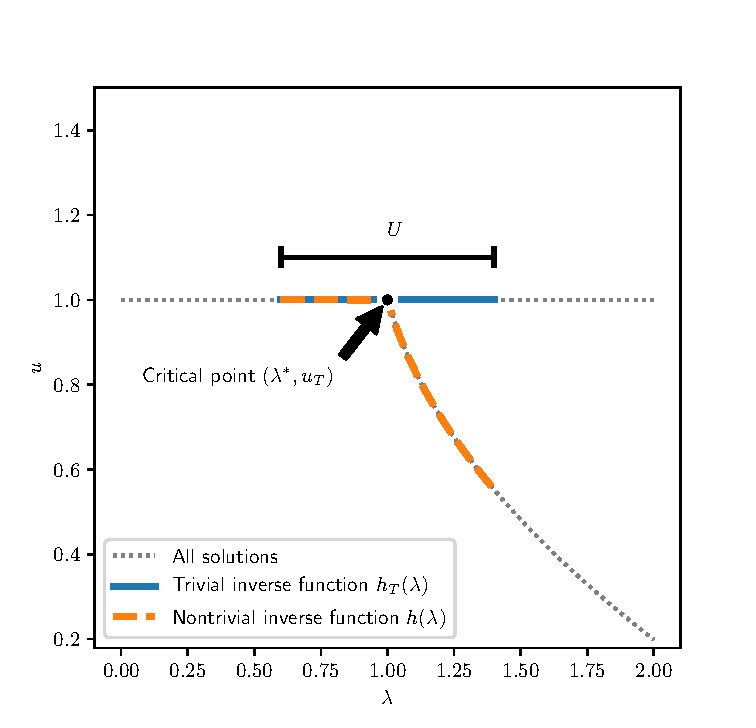
\includegraphics[height=0.35\textwidth]{scheme_continuous_phase_transition}}\hfill
	\sidesubfloat[]{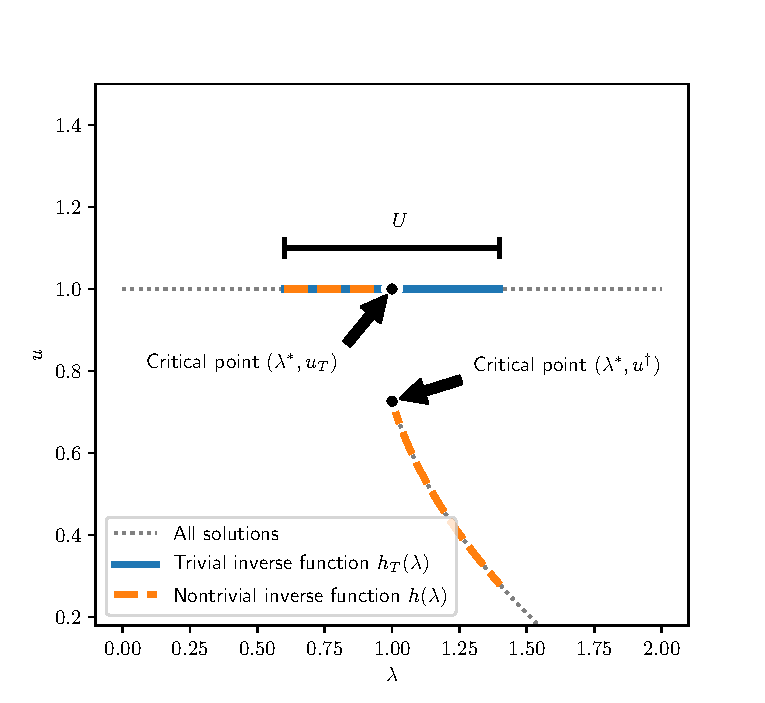
\includegraphics[height=0.35\textwidth]{scheme_discontinuous_phase_transition}}
	\caption{(a) Scheme of a continuous phase transition. (b) Scheme of a discontinuous phase transition.}
	\label{Figure: Scheme of continuous and discontinuous phase transitions}
\end{figure}

On the other hand, let consider a discontinuous phase transition at $\lambdavec^*$. For any neighbourhood $U$ of $\lambdavec^*$ there are two sequences $(\lambdavec_n, \uvec_n)$ and $(\etavec_m, \vvec_m)$ with $\lambdavec_n, \etavec_m \in U$ such that
\begin{align}
	\lim_{n \rightarrow \infty} (\lambdavec_n, \uvec_n) &= (\lambdavec^*, \uvec^\dagger) \quad \text{ avec } \uvec^\dagger \neq \uvec_T \\
	\lim_{m \rightarrow \infty} (\etavec_m, \vvec_m) &= (\lambdavec^*, \uvec_T) \\
	F(\lambdavec_n, \uvec_n) &= 0 \quad \forall n \\
	F(\etavec_m, \vvec_m) &= 0 \quad \forall m.
\end{align}
If we assume that an unique continuous function $h$ solving eq. \eqref{Implicit solution for F} exists, we would have
\begin{align}
	h(\lambdavec_n) &= \uvec_n \quad \forall n \\
	h(\etavec_m) &= \vvec_m \quad \forall m.
\end{align}
The continuity of $h$ would furthermore imply
\begin{align}
	h(\lambdavec^*) = \lim_{n \rightarrow \infty} h(\lambdavec_n) = \lim_{n \rightarrow \infty} \uvec_n = \uvec^\dagger,
\end{align}
but also
\begin{align}
	h(\lambdavec^*) &= \lim_{m \rightarrow \infty} h(\etavec_m) = \lim_{m \rightarrow \infty} \vvec_m = \uvec_T.
\end{align}
Since $\uvec_T \neq \uvec^\dagger$, this gives raise to the contradiction $h(\lambdavec^*) \neq h(\lambdavec^*)$. Therefore our assumption must be false and no continuous function $h$ can be defined to solve eq. \eqref{Implicit solution for F}. So finally, we have $\det\left[ J(\lambdavec^*, \uvec^*) \right] = 0$, $\uvec^*$ being either $\uvec_T$ or $\uvec^\dagger$.


\subsection{One dimensional case}

\todo[inline]{Introduce 1D variables more clearly}
If $L = N = 1$, the problem is the classical problem of a one layer network which degree distribution is determined by a single parameter $\lambda$. In that case the Jacobi matrix $J$ reduces to the scalar quantity
\begin{align}
	J(\lambda, u) = \frac{\partial}{\partial u} \left(g_1(u) - u\right) = \frac{\partial g_1(u)}{\partial u} - 1.
\end{align}
Therefore the condition for the boundary $\det J(\lambda, u) = 0$ becomes
\begin{align}
	\frac{\partial g_1(u)}{\partial u} = 1.
\end{align}

This condition was already introduced and verified previously by\missingref{}.

\section{Interval estimation of the critical region}

\subsection{Theoretical foundation}

Let $C \subset \mathcal{R}^L$ be the set of all parameters $\lambdavec$ corresponding to a critical point. This set correspond to the parameters that solve simultaneously eq. \eqref{Multiplex u final} and eq. \eqref{Boundary condition} for some $\uvec \in \unitinterval^L$. In this section we present an alternative and independent method to estimate $C$ in order to verify that eq. \eqref{Multiplex u final} and \eqref{Boundary condition} yield the expected result.

To do so we introduce concepts from \emph{interval arithmetic}\missingref{}. First of all an interval $I$ is defined a set of the form
\begin{align}
	I = \interval{a, b} = \set{x \in \mathbb{R} | a \leq x \leq b}.
\end{align}
The set of all intervals is denoted as $\mathbb{IR}$. The $N$-dimensional equivalent of an interval is an interval box $B$, defined as the Cartesian product of $N$ intervals,
\begin{align}
	B = I_1 \times I_2 \times \cdots \times I_N, \quad I_k \in \mathbb{IR} \quad \forall k = 1, \dots, N
\end{align}
The set of all $N$-dimensional interval boxes is denoted $\mathbb{IR}^N$.

Given a function $\phi : \mathbb{R}^M \rightarrow \mathbb{R}^N$ it is possible\missingref{} to determine a new interval valued function $\Phi : \mathbb{IR}^M \rightarrow \mathbb{IR}^N$ such that
\begin{align}
	x \in B \quad \Rightarrow \quad \phi(x) \in \Phi(B). \label{Definition interval extension}
\end{align}
A function $\Phi$ with this property is called an interval extension of $\phi$. To determine were the critical region is, we would like, in a sense, to solve eq. \eqref{Multiplex u final} and \eqref{Boundary condition}. Several general schemes exist to solve equations in a guaranteed way using intervals\missingref{}, but here we use a simpler algorithm inspired by them and more suited to our present needs.

We define
\begin{align}
	\psi(\lambdavec, \uvec) = F(\lambdavec, \uvec) + \uvec,
\end{align}
with components
\begin{align}
	\psi_j(\lambdavec, \uvec) = 1 - \left[1 - g_1^{(j)}(u_j) \right] \prod_{\substack{i = 1 \\ i \neq j}}^{L}  \left[1 - g_0^{(i)}(u_i) \right].
\end{align}
Also we define $\Psi$ as an interval extension of $\psi$.

Now, let $\uvec^* \in U_0$ be a solution of \eqref{Implicit equation} for some $\lambdavec \in \Lambda$. By the definition of $\psi$ and eq. \eqref{Definition interval extension},
\begin{align}
	F(\lambdavec^*, \uvec^*) = 0 \quad \Rightarrow \quad \uvec^* = \psi(\lambdavec^*, \uvec^*) \in \Psi(\Lambda, U_0).
\end{align}
Therefore if we apply $\Psi(\Lambda, \cdot)$ to an interval box $U_0$ containing a solution, the resulting interval box contains the solution as well. We know that all solutions $\uvec^*$ are contained in $\unitinterval$ by definition of $\uvec$ and thus by iterating the previous argument from $U_0 = \unitinterval$, all solutions are elements of the interval boxes $U_k(\Lambda)$ recursively defined by
\begin{align}
	U_{k+1}(\Lambda) = \Psi(\Lambda, U_k(\Lambda)). \label{Recursion relation for Uk}
\end{align}
Therefore if we find $k$ such that $U_k = \set{\uvec_T}$, we know that the system for any $\lambdavec \in \Lambda$ only admits the trivial solution.

In praxis however, the sequence $U_k$ never converges to exactly the set $\set{\uvec_T}$, we therefore consider the criterion to be met if
\begin{align}
	U_k \subset [1 - \varepsilon, 1]^L, \label{Criterion for trivial region}
\end{align}
for some small tolerance $\varepsilon$.

Furthermore it is possible in some cases to guarantee the presence of non trivial solutions, allowing to conclude that a GVC emerges. Indeed, if we can find some interval boxes $\Lambda$ and $U$ such that
\begin{align}
	\Psi(\Lambda, U) \subset U \quad \text{and} \quad \uvec_T \notin U, \label{Criterion for non trivial solution}
\end{align}
then by definition of the interval extension (eq. \eqref{Definition interval extension}), we have
\begin{align}
	\psi(\lambdavec, U) \subset U, \quad \forall \lambdavec \in \Lambda.
\end{align}
Since $U$ is closed and simply connected, the fixpoint theorem \todo{Find back which one exactly}\missingref{} applies, implying that for each $\lambdavec \in \Lambda$ there must be at least one $\uvec^*$ in $U$ such that $\uvec^*$ is a fixpoint, or in other words such that $\uvec^* = \psi(\lambdavec, \uvec^*)$. Therefore eq. \eqref{Criterion for non trivial solution} is a sufficient condition to prove the existence of at least one solution. Moreover since we imposed $\uvec_T \notin U$, the solution present can not be the trivial one.

\subsection{Algorithm}

Equations \eqref{Criterion for trivial region} and \eqref{Criterion for non trivial solution} give guaranteed criteria for respectively the absence and presence of a non trivial solution in the region $\Lambda$ considered. This is sufficient to propose an algorithm to estimate the critical region $C$.

\begin{enumerate}
	\item Choose a starting parameter region $\Lambda_0$ and store it in the set $S_{work}$ of regions yet to be processed.
	\item If $S_{work}$ is empty terminate, otherwise retrieve the next parameter region from $S_{work}$, and call it $\Lambda$.
	\item If the radius of $\Lambda$ is smaller than some tolerance $\delta$, store it in the set $S_{unkown}$ of regions for which the algorithm is unable to conclude using the tolerance $\delta$.
	\item Compute $U_k(\Lambda)$ for $k$ big, using eq. \eqref{Recursion relation for Uk}.
	\item If $U_k(\Lambda)$ fulfil eq. \eqref{Criterion for trivial region}, store $\Lambda$ in the set $S_{trivial}$ of trivial regions and go to 2.
	\item Take a subset $V$ of $U_k(\Lambda)$ such that $\uvec_T \notin V$.
	\item If $V$ fulfil eq. \eqref{Criterion for non trivial solution}, store $\Lambda$ in the set $S_{GVC}$ of non trivial regions and go to 2.
	\item Bisect $\Lambda$ in two sub regions and add both to $S_{work}$. Go to 2.
\end{enumerate}

By construction, when the algorithm terminates, we have for the critical region $C$
\begin{align}
	C \subset \bigcup_{U \in S_{unkown}} U,
\end{align}
thus providing an estimation of $C$. For the estimation of $C$ to be faitfull, it is crucial for the interval extension $\Psi$ to be the tightest possible. To get good result in that regard, we used the interval arithmetic implementation of the \code{IntervalArithmetic.jl} Julia package\missingref{}.

\section{Results}

We apply the two methods presented to different cases of multiplex network in order to test it. The algorithm using interval arithmetic is compared to the numerical solution of the system composed by eq. \eqref{Multiplex u final} and \eqref{Boundary condition}, computed using the \code{NLsolve.jl} Julia package.

\todo[inline]{Choose what multiplex networks should be used and with what parameters and actually produce the results.}

\begin{figure}
	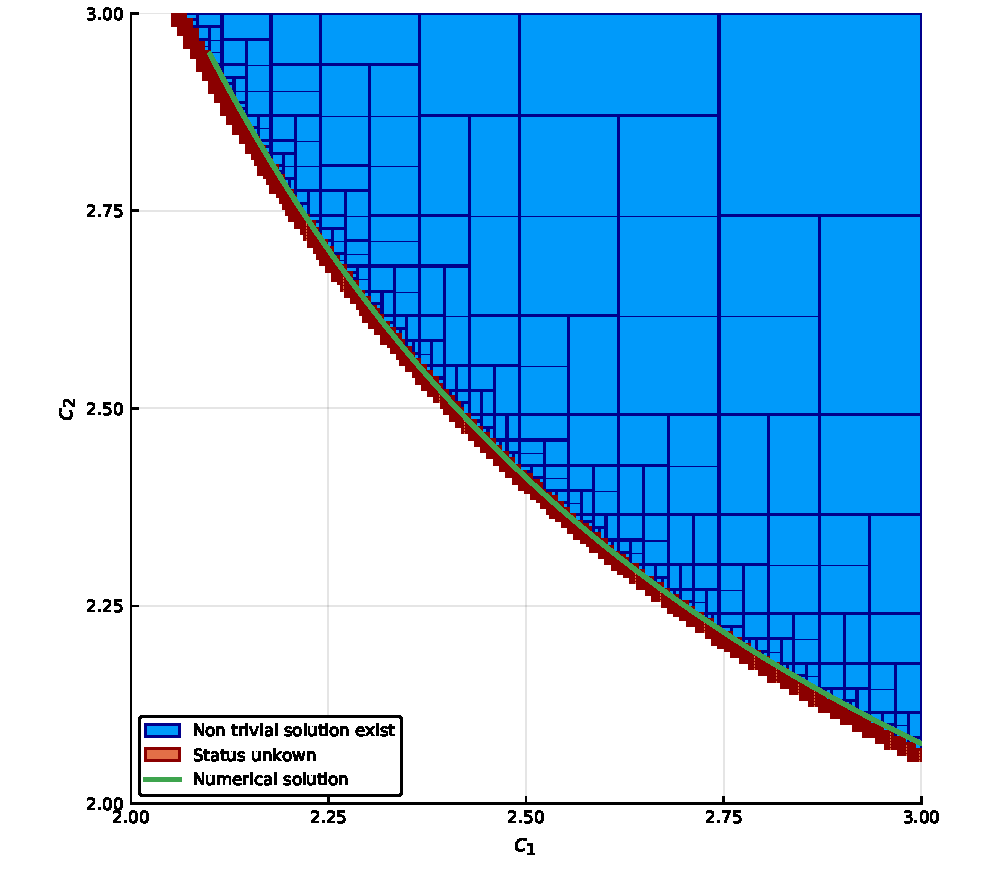
\includegraphics[width=0.8\textwidth]{two_layers_erdos_renyi_boundary.pdf}
	\caption{Phase diagram for a multiplex network composed of two Erdos-Renyi layer with mean degree $c_1$ and $c_2$. In the blue region a non trivial solution for $\uvec$ has been found, in the uncolored region only the trivial solution $\uvec_T$ exists and in the red region the algorithm was unable to conclude in favor of either case. The solid green line is the numerical solution to eq. \eqref{Multiplex u final} and \eqref{Boundary condition}.}
	\label{Figure: Regions and boundary}
	\todo[inline]{Make the plot more readable and less ugly}
	\todo[inline]{Find why the two methods seems drift away one from the other far from the center.}
\end{figure}

\section{Discussion}

\todo[inline]{Write discussion}

\end{document}